 \section{Architecture finale}

  \subsection{Architecture}
  \begin{figure}[!ht]
   \begin{center}
    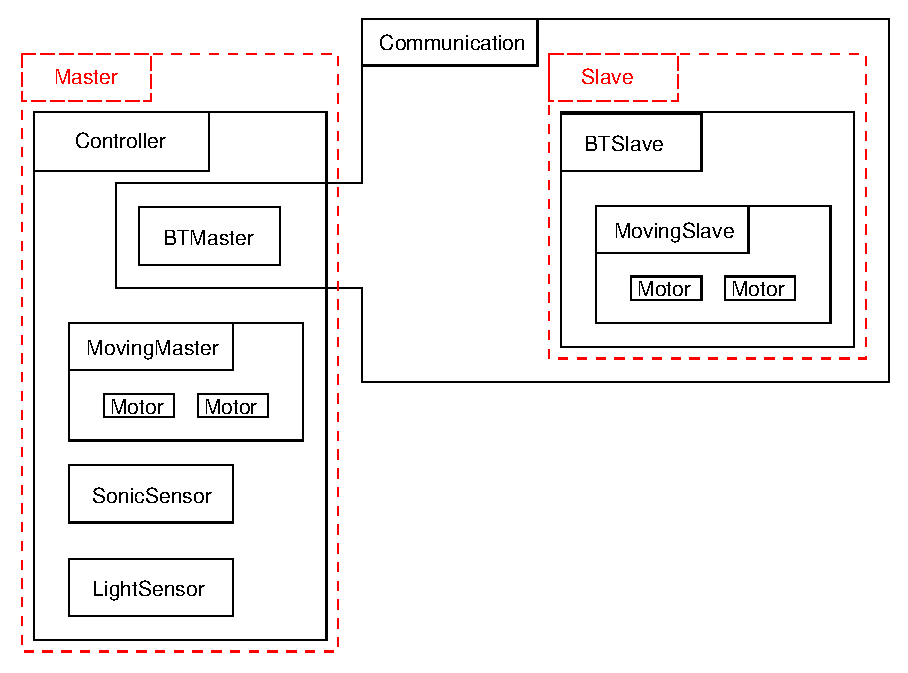
\includegraphics{ARmodel.eps}
    \caption{Architecture AltaRica}
   \end{center}
  \end{figure}

  \subsection{Le n\oe{}ud LightSensor}

   \subsubsection{Description}
   Ce noeud correspond au capteur de lumière, et possède une variable
   d'état nommée $color$ qui   peux prendre trois valeurs différentes,
   correspondants au trois couleurs de case que nous allons utiliser:
   Noir, gris et blanc. Cette variable d'état n'est présente que pour
   pouvoir modéliser des événements, qui seront déclenché par les
   différentes valeurs de la variable de flux $value$. L'action du
   senseur de lumière est donc véritablement représentée par cette
   variable de flux, puisque les valeurs lues par le senseur sont
   "incontrôlables".

   \subsubsection{Le source Altarica}
   \verbatiminput{../src/altarica/alt/LightSensor.alt}
   
   \subsubsection{La spécification}
   \verbatiminput{../src/altarica/acheck/LightSensor.acheck}

   \subsubsection{La sémantique}
%    \begin{figure}[!ht]
%     \begin{center}
%      \includegraphics{../src/altarica/LightSensor.eps}
%     \end{center}
%    \end{figure}
   
  \subsection{Le n\oe{}ud UltraSonicSensor}
  
   \subsubsection{Description}
   De la même manière que le noeud LightSensor, UltraSonicSensor
   comporte une variable d'état "behind" qui servira à pouvoir
   déclencher les deux évènements $readValue$. Le principe du capteur
   est que soit il y a un objet capté, soit il n'y en a pas, sans
   distinction véritable de distance. Et comme pour LightSensor, c'est
   la variable de flux $d$ qui déclenche ces évènements.

   \subsubsection{Le source Altarica}
   \verbatiminput{../src/altarica/alt/UltraSonicSensor.alt}
   
   \subsubsection{La spécification}
   \verbatiminput{../src/altarica/acheck/UltraSonicSensor.acheck}
   
   \subsubsection{La sémantique}
%    \begin{figure}[!ht]
%     \begin{center}
%      
\includegraphics{../src/altarica/UltraSonicSensor.eps}
%     \end{center}
%    \end{figure}

  \subsection{Le n\oe{}ud Motor}
  
   \subsubsection{Description}
   Les moteurs sont modélisés de façon à avoir seulement trois vitesses
   possible: Avancer, stopper, reculer.

   \subsubsection{Le source Altarica}
   \verbatiminput{../src/altarica/alt/Motor.alt}
   
   \subsubsection{La spécification}
   \verbatiminput{../src/altarica/acheck/Motor.acheck}
   
   \subsubsection{La sémantique}
%    \begin{figure}[!ht]
%     \begin{center}
%      \includegraphics{../src/altarica/Motor.eps}
%     \end{center}
%    \end{figure}

  \subsection{Le n\oe{}ud Moving}

   \subsubsection{Description}
   Moving est la pour faire la synchronisation entre les deux moteurs
   munis de roues d'un robot. Il y a cinq ordres possible: Avancer,
   s'arrêter, reculer, à droite et à gauche. Il faut savoir que les
   rotations à droite et à gauche du robot sont tout le temps de 90
   degrés.

   \subsubsection{Le source Altarica}
   \verbatiminput{../src/altarica/alt/Moving.alt}
   
   \subsubsection{La spécification}
   \verbatiminput{../src/altarica/acheck/Moving.acheck}
 
   \subsubsection{La sémantique}
%    \begin{figure}[!ht]
%     \begin{center}
%      \includegraphics[width=16cm]{../src/altarica/Moving.eps}
%     \end{center}
%    \end{figure}

  \subsection{Les n\oe{}uds BTMaster, BTSlave et MasterSlave}
  
   \subsubsection{Description}
   La communication bluetooth entre les deux robots est de type
   maitre/esclave, le maitre envoie simplement des ordres à executer à
   l'esclave. Le noeud BTMaster qui sera pour le robot maitre comporte
   donc simplement les cinq même ordres que le noeud moving. BTSlave
   sera lui pour le robot esclave, et inclus un sous noeud de type
   Moving, afin de pouvoir synchroniser les cinq ordres possibles à un
   agissement concret de ce noeud Moving. Enfin, le noeud MasterSlave se
   chargera de faire la synchronisation entre les ordres des noeuds
   BTMaster et BTSlave.

   \subsubsection{Les sources Altarica}
   \verbatiminput{../src/altarica/alt/BTMaster.alt}
   \verbatiminput{../src/altarica/alt/BTSlave.alt}
   \verbatiminput{../src/altarica/alt/BTMasterSlave.alt}
   
   \subsubsection{Les spécifications}
   \verbatiminput{../src/altarica/acheck/BTMaster.acheck}
   \verbatiminput{../src/altarica/acheck/BTSlave.acheck}
   \verbatiminput{../src/altarica/acheck/BTMasterSlave.acheck}

%    \subsubsection{La sémantique}
%    \begin{figure}[!ht]
%     \begin{center}
%      \includegraphics{../src/altarica/BTMaster.eps}
%      \includegraphics{../src/altarica/BTSlave.eps}
%      \includegraphics{../src/altarica/BTMasterSlave.eps}
%     \end{center}
%    \end{figure}
   
  \subsection{Le n\oe{}ud Controller}
   
   \subsubsection{Les sources Altarica}
   \verbatiminput{../src/altarica/alt/Controller.alt}
